\mychapter{Probabilitat i distribucions de probabilitat}{Probabilitat}{
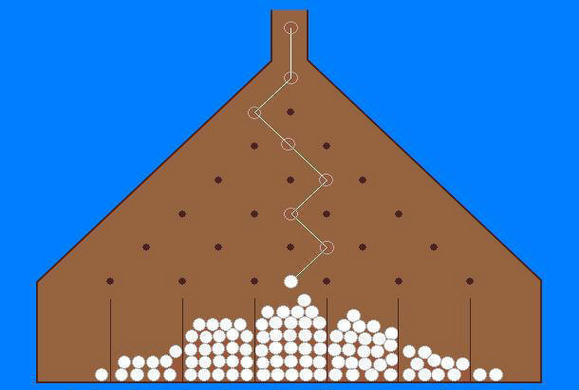
\includegraphics[width=4cm]{img-12/galton}

Màquina de Galton
}{chap:probabilitat}

\section{Axiomatica de la probabilitat}

Anem a veure diferents formes d'assignar probabilitats de successos:

\begin{theorybox}[Llei dels grans nombres]
	Una forma és repetir un experiment moltes vegades i fixar-se en les freqüències relatives $f_r = \frac{f}{N}$. La freqüència relativa és la freqüència absoluta dividit pel nombre de repeticions $N$. La llei dels grans nombres assegura que
	 \begin{equation}
		P(S) = \limx[N]{\infty} \dfrac{\text{freqüència de S}}{N}
	\end{equation}
\end{theorybox}
 
\begin{theorybox}[Regla de Laplace]
 	 
 	\begin{wrapfigure}{R}{0.2\textwidth} 
 		\vspace{-1cm}
 		\begin{center}
 			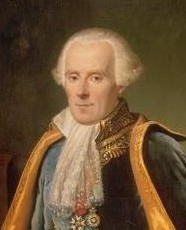
\includegraphics[width=0.16\textwidth]{img-12/laplace}
 			\par \footnotesize Pierre S. Laplace (1749-1827) 
 		\end{center}
 	\end{wrapfigure}
 
   Si  tots els possibles resultats d'un experiment aleatòri són equiprobables (experiència regular), podem assignar probabilitats mitjançant la regla de Laplace; la probabilitat que ocorri el succés $S$ és
   \begin{equation}
   	P(S) = \dfrac{\text{Casos favorables a } S}{\text{Casos totals}}
   \end{equation}
   \vspace{1cm}
\end{theorybox}
\newpage
\begin{theorybox}[Forma axiomàtica]
	Podem definir la nostra pròpia probabilitat seguint una sèrie de regles bàsiques. Si tenim un experiment format pels següents successos elementals $E=\{S_1, S_2, \cdots, S_n\}$, les seves probabilitats $P_i$ han de complir que
	\begin{enumerate}
		\item $0\leq P_i \leq 1$: Les probabilitats estan compreses entre 0 i 1. Si $P(S)=0$, $S$ és el succés impossible i si $P(S)=1$, $S$ és el succés segur.
		
		\item $P_1+P_2+\cdots+P_n=1$: Totes les probabilitats dels successos elementals sumen 1.
		
		\item Definim un succés com un subconjunt de l'espai mostral $S \subseteq E$. Dos successos $S_1$ i $S_2$ són incompatibles si $S_1 \cap S_2 = \emptyset$. S'ha de complir que $P( S_1 \cup S_2)= P(S_1)+P(S_2)$.
		
	\end{enumerate}
\end{theorybox}

\begin{mylist}
	\item
	Escriu el conjunt de possibles resultats de l'experiment aleatori:
	``\emph{Escriure en cinc targetes cadascuna de les vocals i treure una
		a l'atzar}''.
	\item
	Escriu tres successos aleatoris de l'experiment aleatori treure una
	carta d'una baralla espanyola. 
	\item
	Sigui A el succés tirar un dau i treure un nombre major que 4. Escriu
	el succés contrari de A .
	\item
	Calcula la probabilitat que en treure una carta de la baralla sigui
	una espasa.
	\item
	Quina és la probabilitat de \emph{no} treure un 5 en tirar un dau? I
	de \emph{no} treure un múltiple de 3? I de \emph{no} treure un nombre
	menor que 2? 
\end{mylist}

\section{Càlcul de probabilitats}

\begin{theorybox}
	Dos successos $A$ i $B$ són \textbf{independents} si
	\begin{equation*}
	P(A \cap B) = P(A)\cdot P(B)
	\end{equation*}
	
	
	Es defineix la \textbf{probabilitat} de $A$ \textbf{condicionada} que hagi passat $B$ com
	\begin{equation*}
	P(A | B) = \frac{P(A\cap B)}{ P(B)}
	\end{equation*}
	
	Aleshores, si dos successos $A$ i $B$ són \textbf{dependents}
	\begin{equation*}
	P(A \cap B) = P(B)\cdot P(A | B)
	\end{equation*}
	
\end{theorybox}
 

\begin{mylist}
\item
En tirar una moneda dues vegades, quin és la probabilitat de no treure
cap cara? I de treure almenys una cara? Observa que treure almenys una
cara és el succés contrari de no treure cap cara.
\item
En l'experiment ``treure tres cartes seguides'', quina és la
probabilitat de \emph{treure tres asos}? Primer amb reemplaçament, i
després sense reemplaçament.
\item
En tirar dues vegades un dau calcula la probabilitat que surti un sis
doble. 
\item
En tirar dues vegades un dau calcula la probabilitat de treure almenys
un 6. \emph{Ajuda}: Potser et sigui més fàcil calcular la probabilitat
de \emph{no treure cap} 6, i utilitzar el succés contrari.
\item
Llancem dos daus que no estiguin trucats i anotem els nombres de la
seva cara superior. Considerem el succés \emph{A que} la suma de les
dues cares sigui 8, i el succés \emph{B} que aquests nombres
difereixin en dues unitats. a) Comprova que \emph{P}(\emph{A}) = 5/36
(\emph{casos favorables}: 2 + 6; 3 + 5; 4 + 4; 5 + 3; 6 + 2) i que
\emph{P}(\emph{B}) = 8/36 (\emph{casos favorables}: (1, 3), (2, 4),
\ldots{}). 
\item
Dibuixa en el teu quadern un diagrama en arbre per a tres incendis, i
calcula la probabilitat que almenys un hagi estat intencionat essent
la probabilitat d'un incendi \emph{P}(\emph{I}) = 0'6.
\item
En una aeronau s'han instal·lat tres dispositius de seguretat:
\emph{A} \emph{, B} i \emph{C}. Si falla \emph{A} es posa \emph{B} en
funcionament, i si també falla \emph{B} comença a funcionar \emph{C}.
Les probabilitats que funcioni correctament cada dispositiu són:
\emph{P}(\emph{A}) = 0'96; \emph{P}(\emph{B}) = 0'98 i P (\emph{C}) =
0'99. a) Calcula la probabilitat que fallin els tres dispositius. b)
Calcula la probabilitat que tot vagi bé.
\item
Una fàbrica de joguines rebutja normalment el 0'3 \% de la seva
producció per fallades degudes a l'atzar. Calcula la probabilitat que:
a) En agafar dues joguines a l'atzar calgui rebutjar ambdues. b) En
agafar dues joguines a l'atzar calgui rebutjar només una. c) En agafar
dues joguines a l'atzar no calgui rebutjar cap. 
\item
Es tenen 3 caixes, A, B i C. La caixa A té 10 boles de les quals 4 són
negres. La caixa B té 6 boles amb una bola negra. La caixa C té 8
boles amb 3 negres. S'agafa una caixa a l'atzar i d'aquesta caixa es
treu una bola, també a l'atzar. Comprova que la probabilitat que la
bola sigui negra és 113/360.
\item
Tenim una moneda trucada la probabilitat de la qual d'obtenir cara és
3/5 i la de creu és 2/5. Si surt cara s'escull a l'atzar un nombre de
l'1 al 8, i si surt creu, s'escull un nombre de l'1 al 6. Calcula la
probabilitat que el nombre escollit sigui imparell. I PR
\item
Antoni, Joan i Jordi tenen una prova de natació. Antoni i Joan tenen
la mateixa probabilitat de guanyar, i doble a la probabilitat de
Jordi. Calcula la probabilitat que guanyi Joan o Jordi.
\item
Llancem dos daus i anotem els valors de les cares superiors. Calcula
les probabilitats que la suma sigui 1, sigui 2, sigui 3, \ldots{}.
sigui 12.
\item
Llancem una moneda 50 vegades, què és més probable, obtenir 50 cares
seguides o obtenir en les primeres 25 tirades cara i en les 25
següents creu? Raona la resposta.
\item
Una moneda està trucada. La probabilitat d'obtenir cara és doble que
la d'obtenir creu. Calcula les probabilitats dels successos obtenir
cara i d'obtenir creu en tirar la moneda.
\item
Tenim un dau trucat de manera que els nombres imparells tenen una
probabilitat doble a la dels nombres parells. Calcula les
probabilitats de: A) Surti un nombre imparell. B) Surti un nombre
primer. C) Surti un nombre primer imparell. D) Surti un nombre que
sigui primer o sigui imparell.
\item
En un grup de 12 amigues hi ha 3 rosses. Es trien dues noies a
l'atzar. Calcula la probabilitat que: A) Ambdues siguin rosses. B)
Almenys una sigui rossa. C) Cap sigui rossa. D) Una sigui rossa i
l'altra no.
\item
Llancem dos daus i anotem els valors de les cares superiors. Calcula
les probabilitats que: A) Els nombres obtinguts siguin iguals. B) Els
nombres obtinguts difereixin en 3 unitats. C) Els nombres obtinguts
siguin parells.
\item
Llancem una moneda fins que surti cara. Calcula la probabilitat que:
A) Surti cara abans del quart llançament. B) Surti cara després del
vuitè llançament.
\item
Un lot de 20 articles té 2 defectuosos. Es treuen 4 a l'atzar, quin és
la probabilitat que cap sigui defectuós?
\end{mylist}
 

 
\section{La distribució binomial}

\begin{theorybox}[Variable aleatòria]
	Donat un experiment aleatòri amb espai mostral $E=\{S_1, S_2, \cdots, S_n\}$, per a cada succés elemental $S_i$ s'assigna un nombre real $x_i$. Anomenam $x_i$ una variable aleatòria.
	
	Per exemple: Si l'experiment és llançar dues monedes $E=\{CC, CX, XC, XX\}$, podem assignar a cada succés el nombre de cares i tindrem que $x_i$ pot valer 0, 1 o 2 cares.
	
	Cada possible valor de la variable aleatòria $x_i$ tindrà una certa probabilitat $P(x_i)$ que anomenam \textbf{distribució de probabilitat}. 
\end{theorybox}

\begin{theorybox}[Experiència dicotòmica]
	Una experiència és dicotòmica si només poden passar dues coses (o només en fixam en dos aspectes). Per exemple: Èxit/Fracàs, Ploure/No ploure, Aprovar/Suspendre, Cara/Creu, Funciona/No funciona, etc.
\end{theorybox}

\begin{theorybox}[Distribució binomial]
	La binomial és un tipus especial de distribució de variable aleatòria discreta. Sorgeix quan es repeteix una experiència dicotòmica $n$ vegades i les repeticions són \textbf{independents}. A la probabilitat d'èxit la diem $p$ i la de fracàs $q=1-p$.
	 
	Ens demanam quina és la probabilitat que en $n$ repeticions de l'experiment hi hagi $k$ èxits i $n-k$ fracasos.
	
	\begin{equation}
	 P(x=k)=\binom{n}{k} p^k \cdot q^{n-k}
	\end{equation}
	on $\binom{n}{k}$ és el nombre combinatori ''$n$ sobre $k$".
	
	Per a la distribució binomial es compleix que
	\begin{itemize}
		\item 	La mitjana o esperança matemàtica de la variable és $E(x)=\mu = n \cdot p$.
		\item  La desviació típica de la variable és $\sigma = \sqrt{n \cdot p \cdot q}$. 
	\end{itemize}
	
\end{theorybox}

\begin{resolt}[E]{
	Un examen tipus test costa de 10 preguntes, cadascuna d'elles amb 3 opcions de les quals només una és correcta.
	
	 Si contestam l'examen a l'atzar, quina és la probabilitat d'encertar les 10 preguntes? I encertar-ne 5?
	}
	Es tracta d'una binomial de $n=10$ repeticions amb èxit $p=\frac{1}{3}$ i fracàs $q=1-\frac{1}{3}=\frac{2}{3}$; és a dir $B\left(10; \frac{1}{3}\right)$.\vspace{0.25cm}
	
	Encertar les 10 preguntes:\vspace{0.25cm}
	
	 $P(x=10)=\binom{10}{10} \left(\dfrac{1}{3}\right)^{10} \left(\dfrac{2}{3}\right)^{0} = \dfrac{1}{3^{10}} \approx 1.7\times 10^{-5}$.\vspace{0.25cm}
	
	Encertar només 5 preguntes:\vspace{0.25cm}
	
	 $P(x=5)=\binom{10}{5} \left(\dfrac{1}{3}\right)^{5} \left(\dfrac{2}{3}\right)^{5} = 252 \dfrac{2^5}{3^{10}} \approx   0.137$.\vspace{0.25cm}
	 
	 	\begin{wrapfigure}{R}{0.4\textwidth} 
	 	\vspace{-0.25cm}
	 	\begin{center}
	 		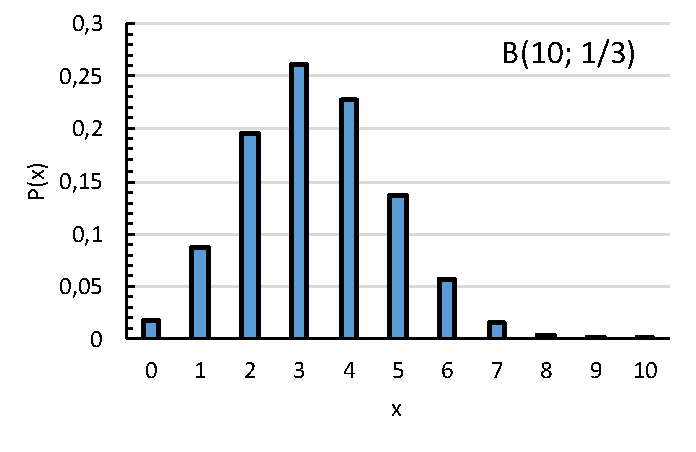
\includegraphics[width=0.4\textwidth]{img-12/binom1}
	 	\end{center}
	  
	 \end{wrapfigure}
 
	 La gràfica mostra la distribució $B\left(10; \frac{1}{3}\right)$, de la qual deduïm que el cas més probable correspon a tenir 3 de 10 preguntes correctes.
	 \vspace{1.5cm}
	
\end{resolt}
\vspace{0.5cm}

\begin{mylist}
	\item
	En una distribució binomial \emph{B}(10, 0'3) calcula
	\emph{P}(\emph{x} = 0), \emph{P}(\emph{x} $\neq$ 0), \emph{P}(\emph{x} = 10) i \emph{P}(\emph{x} = 7). Determina també la mitjana i la desviació típica.
	\item
	Llancem 5 monedes, calcula les probabilitats d'obtenir:
	\begin{tasks}(4)
		\task  0 cares
		\task  1 cara
		\task   2 cares
		\task  3 cares
	\end{tasks}
 
	\item
	Es llança un dau tres vegades i es compta el nombres de tresos que
	apareixen. Es considera la variable aleatòria ``nombre de tresos
	obtinguts''. Representa la distribució de probabilitat. Calcula la
	mitjana i la desviació típica.
	\item
	La població activa d'un cert país es pot dividir en els quals tenen
	estudis superiors i els que no els tenen, sent el primer d'un 20\%.
	Triem 10 persones de la població activa a l'atzar. Escriu l'expressió
	de totes les possibilitats i les seves probabilitats. Calcula la
	probabilitat que hi hagi 9 o 10 que tinguin estudis superiors.
	\item
	S'estima que el percentatge de llars que utilitza una determinada
	marca de tomàquet fregit és del 12\%. En una mostra de 20 llars, quina
	probabilitat hi ha de trobar entre 6 i 15 que ho utilitzin? (No ho
	calculis, només planteja com ho calcularies).
	\item
	Una escola té 500 alumnes 20 dels quals són esquerrans. N'elegim tres
	a l'atzar. Quina és la probabilitat que almenys un sigui esquerrà?
	Suposeu que en cada elecció d'un alumne, la probabilitat que sigui
	esquerrà és la mateixa. 
	\item
	Si la probabilitat que un nen pateixi hemofília és 0,0001, quina és la
	probabilitat que hi hagi al menys un nen hemofílic en una escola que
	té 500 alumnes? 
	\item
	La probabilitat de contreure una malaltia per contacte amb una persona
	malalta és de 2/3. Calculeu la probabilitat de contreure-la que té una
	persona sana que s'exposa a contacte successiu de dos malalts. 
	\item
	La probabilitat que els cargols que fabrica una determinada empresa
	siguin defectuosos és del 10\%, però que un cargol sigui defectuós és
	independent del fet que un altre ho sigui o no. Els cargols
	s'empaqueten en capses de 5 unitats. Calculeu quina probabilitat
	tindrem que en una capsa no hi hagi cap cargol defectuós. 
	\item
	El 20\% d'un model de bombetes és defectuós. En una mostra de 5
	bombetes, calculeu la probabilitat que exactament dues bombetes siguin
	defectuoses. 
	\item
	El 4\% dels USB d'ordinador que fabrica una determinada empresa
	resulten defectuosos. Els USB es distribueixen en capses de 5 unitats.
	Calculeu la probabilitat que en una capsa no hi hagi cap disquet
	defectuós. 
	\item
	La probabilitat que un tirador amb arc faci diana és 0,2. Si fa 5
	intents independents, calculeu la probabilitat que faci exactament 3
	dianes. 
	\item
	Llancem dues monedes i anotam el nombre de cares. Calcula la mitjana i
	la desviació típica d'aquest experiment.
	\item
	Considera l'experiment de llançar una moneda 3 vegades. Indica les
	següents probabilitats. A) Probabilitat que el nombre de cares sigui
	menor que 1. B) Probabilitat que el nombre de cares sigui menor o
	igual a 1. 
	\item
	Calcula la probabilitat que en llançar una moneda 15 vegades el nombre
	de cares sigui menor que 5.
	\item
	Escriu l'expressió (no ho calculis) de la probabilitat que en llançar
	un dau 15 vegades el nombre de cincs sigui major que 10.
	\item
	En el control de qualitat de bombetes de baix consumeix d'una fàbrica
	s'ha comprovat que el 90\% són bones. Es pren una mostra de 500
	bombetes. De mitjana, quantes seran de bona qualitat? Calcula la
	mitjana, variància i desviació típica. 
	\item
	En l'estudi sobre una nova medicina per a l'hepatitis C s'ha comprovat
	que produeix curacions completes en el 80\% dels casos tractats.
	S'administra a mil nous malalts, quantes curacions esperarem que es
	produeixin?
	\item
	S'ha comprovat que la distribució de probabilitat del sexe d'un nounat
	és:
	
	
	\begin{longtable}[]{@{}lll@{}}
		\toprule
		Sexe del nounat: & noia & noi\tabularnewline
		Probabilitat: & 0'485 & 0'515\tabularnewline
		\bottomrule
	\end{longtable}
	En un hospital van nèixer 10 infants. Calcula la probabilitat que neixin 7 noies.
	
\end{mylist}

\vspace{2cm}
\section{La distribució normal}

\begin{theorybox}
		\begin{wrapfigure}{R}{0.4\textwidth} 
		\vspace{-0.25cm}
		\begin{center}
			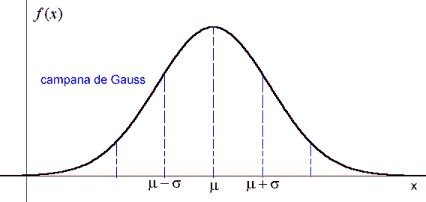
\includegraphics[width=0.4\textwidth]{img-12/campana_gauss1}
		\end{center}
		
	\end{wrapfigure}

	La distribució normal és un tipus especial de distribució de probabilitat de variable contínua. Té com a funció densitat de probabilitat la corba normal o de Gauss
	\begin{equation*}
			f(x)=\frac{1}{\sigma\sqrt{2\pi}}\; e^{ - \frac{1}{2} \left(\frac{x-\mu}{\sigma}\right)^2} 
	\end{equation*}
	on $\mu$ és la mitjana i $\sigma$ és la desviació típica de la distribució $N(\mu; \sigma)$.
	
	Si prenem $\mu=0$ i $\sigma=1$, obtenim la normal estàndard $N(0,1)$. Els valors de les àrees sota aquesta corba estan calculats en la taula de la pàgina \pageref{tab:normal01}. 
\end{theorybox}

\begin{theorybox}[Probabilitats a partir de $N(0,1)$]
	Quan treballam amb la normal estàndard, habitualment empram la lletra $z$ com a variable. 
	
	Considerem $a\geq 0$:
	
	\begin{itemize}
		\item Per a qualsevol variable aleatòria contínua $P(z=a)=0$
		\item $P(z<a)$ és l'àrea sota la corba $N(0,1)$ que estan calculats en la taula de la pàgina \pageref{tab:normal01}. 
		\item $P(z>a)=1-P(z<a)$
		\item $P(z<-a)=P(z>a)=1-P(z<a)$
		\item $P(a<z<b)=P(z<b)-P(z<a)$
		\item $P(-a<z<a)=2P(z<a)-1$
	\end{itemize}	
	
	
	  
	  
\end{theorybox}

\begin{theorybox}[Probabilitats a partir de $N(\mu, \sigma)$]
	En la majoria de casos, ni la mitjana és zero ni la desviació típica és 1. Per calcular probabilitats necessitam tipificar la variable, convertint-la de $x \rightarrow z$
	\begin{equation*}
	 	z=\frac{x-\mu}{\sigma} 
	\end{equation*}
	 Si $x$ segueix una distribució $N(\mu; \sigma)$, la nova variable $z$ segueix una distribució $N(0,1)$ i per tant podem seguir utilitzant la taula de la normal estàndard. 
\end{theorybox}



\begin{mylist}
	\item
	Calcula en una distribució normal estàndard les probabilitats
	següents: 
	\begin{tasks}(4)
		\task \emph{P}(\emph{z} = 0)
		\task \emph{P}(\emph{z} \textless{} 0)
		\task \emph{P}(\emph{z} = 1'82)
		\task \emph{P}(\emph{z} \textgreater{} 1'82)
	\end{tasks}
	
	\item
	Calcula en una distribució normal estàndard les probabilitats
	següents: 
	\begin{tasks}(4)
		\task \emph{P}(\emph{z} \textgreater{} 4)
		\task \emph{P}(\emph{z}
		\textless{} 4)
		\task \emph{P}(\emph{z} \textgreater{} 1)
		\task \emph{P}(\emph{z} \textless{} 1)
	\end{tasks} 
\end{mylist}

\vspace{2cm}

\begin{resolt}[E]{Les estatures es distribueixen segons una normal de mitjana 175 cm i desviació típica 10 cm. Calcula la probabilitat que un individu: \vspace{0.2cm}
		
\hspace{-1cm}\begin{enumerate}
	\item[a)] mesuri més que 180 cm
	\item[b)] mesuri menys que 170 cm
	\item[b)] la proporció d'individius amb altura compresa entre 170 i 180 cm
\end{enumerate}	
}
	L'estatura $x$ segueix una normal $N(\mu=170, \sigma=10)$ \vspace{0.25cm}
	
	a) $P(x>180)=P\left[ z>\dfrac{180-175}{10} \right]=P\left[x>0.5\right]=1-P\left[z<0.5\right]=1-0.6915=0.3085$ \vspace{0.25cm}
	
	b) $P(x<170)=P\left[ z<\dfrac{170-175}{10} \right]=P\left[x<-0.5\right]=1-P\left[z<0.5\right]=1-0.6915=0.3085$\vspace{0.25cm}
	
	c) $P(170<x<180)=P\left[ -0.5 < z< 0.5 \right]=2P\left[x<0.5\right]-1=2\cdot 0.3085 -1=0.383$. Aleshores el 38.5\% dels individius tenen estatures entre 170 i 180 cm.
\end{resolt}
\vspace{1cm}

\begin{table}[t]
	\label{tab:normal01}
	\begin{center}
		\Large	\textbf{Àrees sota la distribució normal estàndard, N(0,1)}
		
		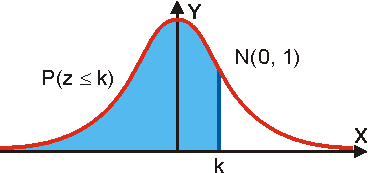
\includegraphics[width=5cm]{img-12/normal01}
	\end{center}
	\vspace{0.25cm}
	
	\centering
	\begin{tabular}{r|rrrrr|rrrrr}
		\hline
		$z$ & 0 & 0.001 & 0.002 & 0.003 & 0.004 & 0.005 & 0.006 & 0.007 & 0.008 & 0.009 \\ 
		\hline
		\rowcolor{lightgray} 0 & 0.5000 & 0.5040 & 0.5080 & 0.5120 & 0.5160 & 0.5199 & 0.5239 & 0.5279 & 0.5319 & 0.5359 \\ 
		0.1 & 0.5398 & 0.5438 & 0.5478 & 0.5517 & 0.5557 & 0.5596 & 0.5636 & 0.5675 & 0.5714 & 0.5753 \\ 
		\rowcolor{lightgray}0.2 & 0.5793 & 0.5832 & 0.5871 & 0.5910 & 0.5948 & 0.5987 & 0.6026 & 0.6064 & 0.6103 & 0.6141 \\ 
		0.3 & 0.6179 & 0.6217 & 0.6255 & 0.6293 & 0.6331 & 0.6368 & 0.6406 & 0.6443 & 0.6480 & 0.6517 \\ 
		\rowcolor{lightgray}0.4 & 0.6554 & 0.6591 & 0.6628 & 0.6664 & 0.6700 & 0.6736 & 0.6772 & 0.6808 & 0.6844 & 0.6879 \\ 
		0.5 & 0.6915 & 0.6950 & 0.6985 & 0.7019 & 0.7054 & 0.7088 & 0.7123 & 0.7157 & 0.7190 & 0.7224 \\ 
		\rowcolor{lightgray}0.6 & 0.7257 & 0.7291 & 0.7324 & 0.7357 & 0.7389 & 0.7422 & 0.7454 & 0.7486 & 0.7517 & 0.7549 \\ 
		0.7 & 0.7580 & 0.7611 & 0.7642 & 0.7673 & 0.7704 & 0.7734 & 0.7764 & 0.7794 & 0.7823 & 0.7852 \\ 
		\rowcolor{lightgray}0.8 & 0.7881 & 0.7910 & 0.7939 & 0.7967 & 0.7995 & 0.8023 & 0.8051 & 0.8078 & 0.8106 & 0.8133 \\ 
		0.9 & 0.8159 & 0.8186 & 0.8212 & 0.8238 & 0.8264 & 0.8289 & 0.8315 & 0.8340 & 0.8365 & 0.8389 \\ 
		\rowcolor{lightgray}1 & 0.8413 & 0.8438 & 0.8461 & 0.8485 & 0.8508 & 0.8531 & 0.8554 & 0.8577 & 0.8599 & 0.8621 \\ 
		1.1 & 0.8643 & 0.8665 & 0.8686 & 0.8708 & 0.8729 & 0.8749 & 0.8770 & 0.8790 & 0.8810 & 0.8830 \\ 
		\rowcolor{lightgray}1.2 & 0.8849 & 0.8869 & 0.8888 & 0.8907 & 0.8925 & 0.8944 & 0.8962 & 0.8980 & 0.8997 & 0.9015 \\ 
		1.3 & 0.9032 & 0.9049 & 0.9066 & 0.9082 & 0.9099 & 0.9115 & 0.9131 & 0.9147 & 0.9162 & 0.9177 \\ 
		\rowcolor{lightgray}1.4 & 0.9192 & 0.9207 & 0.9222 & 0.9236 & 0.9251 & 0.9265 & 0.9279 & 0.9292 & 0.9306 & 0.9319 \\ 
		1.5 & 0.9332 & 0.9345 & 0.9357 & 0.9370 & 0.9382 & 0.9394 & 0.9406 & 0.9418 & 0.9429 & 0.9441 \\ 
		\rowcolor{lightgray}1.6 & 0.9452 & 0.9463 & 0.9474 & 0.9484 & 0.9495 & 0.9505 & 0.9515 & 0.9525 & 0.9535 & 0.9545 \\ 
		1.7 & 0.9554 & 0.9564 & 0.9573 & 0.9582 & 0.9591 & 0.9599 & 0.9608 & 0.9616 & 0.9625 & 0.9633 \\ 
		\rowcolor{lightgray}1.8 & 0.9641 & 0.9649 & 0.9656 & 0.9664 & 0.9671 & 0.9678 & 0.9686 & 0.9693 & 0.9699 & 0.9706 \\ 
		1.9 & 0.9713 & 0.9719 & 0.9726 & 0.9732 & 0.9738 & 0.9744 & 0.9750 & 0.9756 & 0.9761 & 0.9767 \\ 
		\rowcolor{lightgray}2 & 0.9772 & 0.9778 & 0.9783 & 0.9788 & 0.9793 & 0.9798 & 0.9803 & 0.9808 & 0.9812 & 0.9817 \\ 
		2.1 & 0.9821 & 0.9826 & 0.9830 & 0.9834 & 0.9838 & 0.9842 & 0.9846 & 0.9850 & 0.9854 & 0.9857 \\ 
		\rowcolor{lightgray}2.2 & 0.9861 & 0.9864 & 0.9868 & 0.9871 & 0.9875 & 0.9878 & 0.9881 & 0.9884 & 0.9887 & 0.9890 \\ 
		2.3 & 0.9893 & 0.9896 & 0.9898 & 0.9901 & 0.9904 & 0.9906 & 0.9909 & 0.9911 & 0.9913 & 0.9916 \\ 
		\rowcolor{lightgray}2.4 & 0.9918 & 0.9920 & 0.9922 & 0.9925 & 0.9927 & 0.9929 & 0.9931 & 0.9932 & 0.9934 & 0.9936 \\ 
		2.5 & 0.9938 & 0.9940 & 0.9941 & 0.9943 & 0.9945 & 0.9946 & 0.9948 & 0.9949 & 0.9951 & 0.9952 \\ 
		\rowcolor{lightgray}2.6 & 0.9953 & 0.9955 & 0.9956 & 0.9957 & 0.9959 & 0.9960 & 0.9961 & 0.9962 & 0.9963 & 0.9964 \\ 
		2.7 & 0.9965 & 0.9966 & 0.9967 & 0.9968 & 0.9969 & 0.9970 & 0.9971 & 0.9972 & 0.9973 & 0.9974 \\ 
		\rowcolor{lightgray}2.8 & 0.9974 & 0.9975 & 0.9976 & 0.9977 & 0.9977 & 0.9978 & 0.9979 & 0.9979 & 0.9980 & 0.9981 \\ 
		2.9 & 0.9981 & 0.9982 & 0.9982 & 0.9983 & 0.9984 & 0.9984 & 0.9985 & 0.9985 & 0.9986 & 0.9986 \\ 
		\rowcolor{lightgray}3 & 0.9987 & 0.9987 & 0.9987 & 0.9988 & 0.9988 & 0.9989 & 0.9989 & 0.9989 & 0.9990 & 0.9990 \\
		3.1 & 0.9990 & 0.9991 & 0.9991 & 0.9991 & 0.9992 & 0.9992 & 0.9992 & 0.9992 & 0.9992 & 0.9993 \\  
		\rowcolor{lightgray}3.2 & 0.9993 & 0.9993 & 0.9994 & 0.9994 & 0.9994 & 0.9994 & 0.9994 & 0.9994 & 0.9995 & 0.9995 \\ 
		3.3 & 0.9995 & 0.9995 & 0.9995 & 0.9996 & 0.9996 & 0.9996 & 0.9996 & 0.9996 & 0.9996 & 0.9996 \\ 
		\rowcolor{lightgray}3.4 & 0.9997 & 0.9997 & 0.9997 & 0.9997 & 0.9997 & 0.9997 & 0.9997 & 0.9997 & 0.9997 & 0.9997 \\ 
		3.5 & 0.9998 & 0.9998 & 0.9998 & 0.9998 & 0.9998 & 0.9998 & 0.9998 & 0.9998 & 0.9998 & 0.9998 \\ 
		\rowcolor{lightgray}3.6 & 0.9998 & 0.9998 & 0.9999 & 0.9999 & 0.9999 & 0.9999 & 0.9999 & 0.9999 & 0.9999 & 0.9999 \\ 
		3.7 & 0.9999 & 0.9999 & 0.9999 & 0.9999 & 0.9999 & 0.9999 & 0.9999 & 0.9999 & 0.9999 & 0.9999 \\ 
		\rowcolor{lightgray}3.8 & 0.9999 & 0.9999 & 0.9999 & 0.9999 & 0.9999 & 0.9999 & 0.9999 & 0.9999 & 0.9999 & 0.9999 \\ 
		3.9 & 1.0000 & 1.0000 & 1.0000 & 1.0000 & 1.0000 & 1.0000 & 1.0000 & 1.0000 & 1.0000 & 1.0000 \\ 
		\rowcolor{lightgray}	4.0 & 1.0000 & 1.0000 & 1.0000 & 1.0000 & 1.0000 & 1.0000 & 1.0000 & 1.0000 & 1.0000 & 1.0000 \\ 
		\hline
	\end{tabular}
\end{table}


\begin{mylist}
 
	 
	\item
	Calcula en una distribució normal estàndard les probabilitats
	següents: 
	  	\begin{tasks}(2)
	 	\task \emph{P}(1 \textless{} \emph{z \textless{} }2)
	 	\task \emph{P}(--1'3
	 	\textless{} \emph{z} \textless{} 4)
	 	\task \emph{P}(--0'2 \textless{}
	 	\emph{z} \textless{} 2'34)
	 	\task \emph{P}(--1 \textless{}\emph{z}
	 	\textless{} 1)
	 \end{tasks} 
 
 
	\item
	Calcula en una distribució normal \emph{N}(1, 2) les probabilitats
	següents: 
	  	\begin{tasks}(4)
	 	\task \emph{P}(\emph{x} \textgreater{} 4)
	 	\task \emph{P}(\emph{x}
	 	\textless{} 4)
	 	\task \emph{P}(\emph{x} \textgreater{} 1)
	 	\task \emph{P}(\emph{x} \textless{} 1)
	 \end{tasks} 
 
	\item
	Calcula en una distribució normal \emph{N}(0'5, 0'2) les probabilitats
	següents: 
	  	\begin{tasks}(4)
	 	\task \emph{P}(\emph{x} \textgreater{} 4)
	 	\task \emph{P}(\emph{x}
	 	\textless{} 4)
	 	\task \emph{P}(\emph{x} \textgreater{} 1)
	 	\task \emph{P}(\emph{x} \textless{} 1)
	 \end{tasks} 
 
 
	\item
	Calcula en una distribució normal \emph{N}(1, 1/2) les probabilitats
	següents:
	 	\begin{tasks}(2)
		\task \emph{P}(1 \textless{} \emph{x \textless{} }2)
		\task \emph{P}(--1'3
		\textless{} \emph{x} \textless{} 4)
		\task \emph{P}(--0'2 \textless{}
		\emph{x} \textless{} 2'34)
		\task \emph{P}(--1 \textless{} \emph{x}
		\textless{} 3)
	\end{tasks} 
	
	\item
	Les alçades de les persones d'una certa població es distribueixen
	segons una normal de mitjana 180 cm i desviació típica 15 cm.
	Determina les probabilitat que: 

\begin{enumerate}
\item Una persona tingui una alçada superior a 190 cm.

\item Una persona tingui una alçada menor a 160 cm.

\item  Quina proporció de persones tenen una alçada compresa entre 160 cm i
190 cm?
\end{enumerate}
 
\item
En un examen per entrar en un cos de l'Estat se sap que els punts
obtinguts es distribueixen segons una normal de mitjana 100 i
desviació típica 10 punts. Determina la probabilitat que:

\begin{enumerate}
\item Un opositor obtingui 120 punts.

\item Si per aprovar és necessari tenir més de 120 punts, Quin percentatge
d'opositors aproven?
\end{enumerate}
 
\item
Es llança una moneda mil vegades, quin és la probabilitat que el
nombre de cares obtingudes estigui entre 400 i 600? I que sigui major
que 800?
\item
En una fàbrica de bombetes de baix consum se sap que el 70\% d'elles
tenen una vida mitjana superior a 1000 hores. Es pren una mostra de 50
bombetes, quin és la probabilitat que hi hagi entre 20 i 30 la vida
mitjana de la qual sigui superior a mil hores?, i la probabilitat que
hi hagi més de 45 la vida mitjana de la qual sigui superior a 1000
hores? 

\item
Una companyia aèria ha estudiat que el 5\% de les persones que
reserven un bitllet per a un vol no es presenten, per la qual cosa
venen més bitllets que les places disponibles. Un determinat avió de
la companyia té 260 places (amb el que solen reservar fins a 270).
Calcula la probabilitat que arribin 260 passatgers. En 500 vols
d'aquest avió, en quants consideres que hi haurà excés de passatgers? 

\item
Es llança 600 vegades un dau i mirem el nombre de 5s. a) Quin és
l'interval simètric respecte de la mitjana amb una probabilitat de
0'99? b) El mateix amb una probabilitat del 0'6. 
 
\end{mylist}


\newpage
\resum

\begin{longtable}[]{|p{4cm}|p{5cm}|p{5cm}|}
	\toprule
	 \cellcolor{lightgray}
		Propietats de la distribució de probabilitat discreta $\{x_i\}$  & 
		\begin{enumerate}
			\item $P(x_i)\geq 0$
			\item $\sum P(x_i) = 1$
		\end{enumerate}
		  &  
		Llancem dues monedes i comptam el nombre de cares:\strut
		
		\begin{tabular}{l|l|l|l}
		$x_i$ & 0 & 1 & 2 \\ \hline \vspace{0.2cm}
		$P(x_i)$ & $\frac{1}{4}$ & $\frac{1}{2}$ & $\frac{1}{4}$
		\end{tabular}
		
		\\ [0.25cm] \hline
		 \cellcolor{lightgray}
		Propietats de funció densitat de probabilitat $f(x)$ & 
		\begin{enumerate}
			\item $f(x) \geq 0$
			\item Àrea sota $f(x)$ és 1
		\end{enumerate} & Exemple: 
	
	$f(x)=\frac{1}{10}$ per a $0\leq x \leq 10$ 
	
  \\ [0.25cm] \hline
   \cellcolor{lightgray}
	Propietats de funció de distribució contínua $F(x)$ & 
	\begin{enumerate}
		\item $0 \leq F(x) \leq 1$
		\item $F(x)$ és una funció creixent
		\item $F(x_{max})=1$
	\end{enumerate} & Exemple: 

$F(x)=\frac{1}{10}x$ per a $0\leq x \leq 10$  \\ \hline
 \cellcolor{lightgray}
	Esperança matemàtica & & $\mu = 0 \cdot (1/4) + 1 \cdot (1/2) + 2 \cdot (1/4) =
	1$ \\ [0.25cm] \hline
	  \cellcolor{lightgray}
		Variància i desviació típica\strut
  &   &  
		$\sigma^2 = (0-1)^2\cdot(1/4) +
		(1-1)^2\cdot(1/2) + (2-1)^2\cdot(1/4) =
		1/2$ 
	 \\ \hline
	  \cellcolor{lightgray}
		Distribució binomial  &  
		$ E(x) = \mu = n\cdot p$,
		
		$\sigma^2 = n \cdot p \cdot (1-p)$ \strut
	  &  
		\emph{B}(10, 1/2). 
		\\[0.25cm] \hline
		 \cellcolor{lightgray}
	Distribució normal & &
	\vspace{0.5cm}
	\begin{center}
	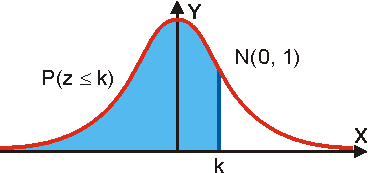
\includegraphics[width=5cm]{img-12/normal01}
	\end{center}
	\\ [0.25cm]\hline
	 \cellcolor{lightgray}
	Aproximació de la binomial a la normal & Una binomial amb $npq \geq 9$
	es considera s'ajusta bé a una normal d'igual mitjana i desviació
	típica. & \\ [0.25cm]\hline
	\bottomrule
\end{longtable}
